\appendixchapheadline % do not modify this unless you really want to
\label{cha:appendix}

% \section{Algorithms for Probability Sampling Methods}
% \label{app:algorithms}

% % The geometric distribution $Geo\left(p\right) $ (cf.~\autoref{def:GeometricDistribution}) generate a random variable $x$ by counting the number of Bernoulli trials up and including the first success (with success probability $p$). \\

% % \subsection{Geometric Distribution}
% % \autoref{algo:Geometric}~\cite{walker1974fast, googleDP2019} generates a geometric random variable $x\sim Geo\left(0.5\right) $ by first generating an $8$-bit random string $r\in \left\{0,1\right\}^8 $ (i.e., eight Bernoulli trials) and counting its leading zeros (i.e., number of trials before the first success) into $x$. If all the bits in $r$ are zeros, an new $8$-bit random string is generated and its leading zeros is also counted into $x$. This process repeats until the random strings contain one (i.e., the first success trial).
% % \begin{algorithm}[tbh!]
% %     \centering
% %     \fbox{
% %         \pseudocode[space=none, syntaxhighlight=auto, addkeywords={Algorithm, Input, Output, IF,TO,RETURN, FOR, ELSE IF, ELSE, WHILE},linenumbering, skipfirstln, head=\textbf{Algorithm: $Algo^{Geo}$}]{
% %             \textbf{Input: None} \pcskipln \\
% %             \textbf{Output: $x\sim Geo\left(0.5\right) $} \\
% %             \text{$x\gets 1$} \\
% %             \text{WHILE $r==0$} \\
% %             \text{\t\t $r\gets Random8bits()$} \\
% %             \text{\t\t $x\gets x+LeadingZeros(r)$} \\
% %             \text{RETURN $x$}
% %         }}
% %     \caption{Algorithm for geometric distribution $x\sim Geo\left(0.5\right)$.}
% %     \label{algo:Geometric}
% % \end{algorithm}
% % \FloatBarrier

% % $Algo^{GeoExp}\left(p=1-e^{\frac{numer}{denom}}\right) $~\cite{canonne2020discrete} generate a random variable $x\sim Geo\left( p=1-e^{\frac{numer}{denom}}\right)$. \\
% % \TODO{prove correctneses}\\
% \begin{algorithm}[tbh!]
%     \centering
%     \fbox{
%         \pseudocode[space=none, syntaxhighlight=auto, addkeywords={Algorithm, Input, Output, IF,TO,RETURN, FOR, ELSE IF, ELSE, WHILE, TRUE, FALSE, CONTINUE,BREAK},linenumbering, skipfirstln, head=\textbf{Algorithm: $Algo^{GeoExp}\left(n,d\right) $}]{
%             \textbf{Input: None} \pcskipln \\
%             \textbf{Output: $x\sim Geo\left( p=1-e^{\frac{n}{d}}\right)$} \\
%             \text{IF $n==0$}\\
%             \text{\t\t RETURN $0$} \\
%             \text{WHILE TRUE}\\
%             \text{\t\t $u \gets Algo^{RandInt}\left(d\right) $}\\
%             \text{\t\t $b_1 \gets Algo^{BernEXP1}\left(u,d\right) $}\\
%             \text{\t\t IF $b_1==1$}\\
%             \text{\t\t \t\t BREAK}\\
%             % geometric (1-exp(-1))
%             \text{$k \gets 0$}\\
%             \text{WHILE TRUE}\\
%             \text{\t\t $b_2\gets Algo^{BernEXP1}\left(1\right) $}\\
%             \text{\t\t IF $b_2==1$}\\
%             \text{\t\t \t\t $k \gets k+1$}\\
%             \text{\t\t ELSE}\\
%             \text{\t\t \t\t BREAK}\\
%             \text{RETURN $x\gets \frac{k\cdot d+u}{n}$}
%         }}
%     \caption{Algorithm for geometric distribution $x\sim Geo\left( p=1-e^{\frac{n}{d}}\right)$~\cite{canonne2020discrete}.}
%     \label{algo:GeometricExp}
% \end{algorithm}
% \FloatBarrier


% % \subsection{Bernoulli Distribution}
% % \begin{algorithm}[tbh!]
% %     \centering
% %     \fbox{
% %         \pseudocode[space=none, syntaxhighlight=auto, addkeywords={Algorithm, Input, Output, IF,TO,RETURN, FOR, ELSE IF, ELSE, WHILE},linenumbering, skipfirstln, head=\textbf{Algorithm: $Algo^{Bern}\left(p\right) $}]{
% %             \textbf{Input: $p$} \pcskipln \\
% %             \textbf{Output: $x\sim Bern\left(p\right) $} \\
% %             \text{$u\gets Uniform\left(0,1\right) $}\\
% %             \text{IF $u<p$}\\
% %             \text{\t\t RETURN $x\gets 1$}\\
% %             \text{ELSE}\\
% %             \text{\t\t RETURN $x \gets 0$}
% %         }}
% %     \caption{Algorithm for Bernoulli distribution $x\sim Bern\left(p\right) $.}
% %     \label{algo:Bernoulli}
% % \end{algorithm}
% % \FloatBarrier

% % $Algo^{BernEXP1}\left(\gamma\right) $~\cite{canonne2020discrete} generates a random variable $x \sim Bern\left( p=e^{-\gamma}\right)$ for $\gamma \in \left[0,1\right] $. $\text{MOD2}\left(j\right) $ outputs $1$ if $j$ is an odd, and $0$ otherwise.\\
% % \TODO{Prove correctness}\\
% \begin{algorithm}[tbh!]
%     \centering
%     \fbox{
%         \pseudocode[space=none, syntaxhighlight=auto, addkeywords={Algorithm, Input, Output, IF,TO,RETURN, FOR, ELSE IF, ELSE, WHILE, TRUE, FALSE, CONTINUE},linenumbering, skipfirstln, head=\textbf{Algorithm: $Algo^{BernEXP1}\left(\gamma\right) $}]{
%             \textbf{Input: $\gamma$} \pcskipln \\
%             \textbf{Output: $x\sim Bern \left( p=e^{-\gamma}\right)$, where $\gamma \in \left[0,1\right] $} \\
%             \text{$j \gets 1$}\\
%             \text{WHILE TRUE}\\
%             \text{\t\t $b\gets Algo^{Bern}\left(\frac{\gamma}{j}\right) $}\\
%             \text{\t\t IF $b==1$}\\
%             \text{\t\t \t\t $j\gets j+1$}\\
%             \text{\t\t ELSE}\\
%             \text{\t\t \t\t BREAK}\\
%             \text{RETURN $x\gets \text{MOD2}\left(j\right) $}
%         }}
%     \caption{Algorithm for Bernoulli distribution $x\sim Bern\left( p=e^{-\gamma}\right)$ with $\gamma \in \left[0,1\right] $~\cite{canonne2020discrete}.}
%     \label{algo:BernoulliEXP1}
% \end{algorithm}
% \FloatBarrier


% % \autoref{algo:BernoulliEXP}~\cite{canonne2020discrete} generates a random variable $x \sim Bern\left( p=e^{-\gamma}\right)$.\\
% % \TODO{Prove correctness}\\
% \begin{algorithm}[tbh!]
%     \centering
%     \fbox{
%         \pseudocode[space=none, syntaxhighlight=auto, addkeywords={Algorithm, Input, Output, IF,TO,RETURN, FOR, TO, ELSE IF, ELSE, WHILE, TRUE, FALSE, CONTINUE},linenumbering, skipfirstln, head=\textbf{Algorithm: $Algo^{BernEXP}\left(\gamma\right) $}]{
%             \textbf{Input: $\gamma$} \pcskipln \\
%             \textbf{Output: $x\sim Bern\left( p=e^{-\gamma}\right)$} \\
%             \text{IF $\gamma \in \left[0,1\right] $}\\
%             \text{\t\t $b_1\gets Algo^{BernEXP1}\left(\gamma\right) $}\\
%             \text{\t\t RETURN $x \gets b_1$}\\
%             \text{ELSE}\\
%             \text{\t\t FOR $j = 0$ TO $ \left\lfloor \gamma\right\rfloor -1 $}\\
%             \text{\t\t \t\t $b_2 \gets Algo^{BernEXP1}\left(1\right)$}\\
%             \text{\t\t \t\t IF $b_2==0$}\\
%             \text{\t\t \t\t \t\t RETURN $x \gets 0$}\\
%             \text{\t\t $b_3\gets Algo^{BernEXP1}\left(\gamma-\left\lfloor \gamma\right\rfloor\right)$}\\
%             \text{RETURN $x\gets b_3$}
%         }}
%     \caption{Algorithm for Bernoulli distribution $x\sim Bern\left( p=e^{-\gamma}\right)$~\cite{canonne2020discrete}.}
%     \label{algo:BernoulliEXP}
% \end{algorithm}
% \FloatBarrier


% \subsection{Random Integer}
% $Algo^{RandInt}\left(m\right)$ uses the Simple Modular Method~\cite{barker2015recommendation} to generate a random integer $x$ such that $0\leq x \leq m-1$. $l$ is the number of bits needed to represent value $m-1$ and $\kappa\geq 64$ is the security parameter.
% % \TODO{security analyse}
% \begin{algorithm}[tbh!]
%     \centering
%     \fbox{
%     \pseudocode[space=none, syntaxhighlight=auto, addkeywords={Algorithm, Input, Output, IF,TO,RETURN, FOR, ELSE IF, ELSE, WHILE, TRUE, FALSE, CONTINUE,BREAK},linenumbering, skipfirstln, head=\textbf{Algorithm: $Algo^{RandInt}\left(m\right)$}]{
%     \textbf{Input: $m$} \pcskipln \\
%     \textbf{Output: $x$} \\
%     \text{Generate random bits $b_0,\ldots,b_{l+\kappa-1}$}\\
%     \text{Calculate $r=\sum_{j=0}^{l+\kappa-1}2^{j}b_{j}$}\\
%     \text{Calculate $x=r \mod{m}$}
%     }}
%     \caption{Algorithm for generate random integer $x \in [0,\ldots,m)$.}
%     \label{algo:RandInt}
% \end{algorithm}
% \FloatBarrier


\section{MPC Protocols}
\label{app:MPCBuildingBlocks}
% \TODO{ABY, share conversion in preliminary part}\\
% ${Pow2}\left(\left\langle \boldsymbol{x}\right\rangle\right) $ calculates $2^{x}$, and the share type of $x$ could be boolean or arthmetic sharings.\\

% \label{prot:PreOr}
% Protocol $\Uppi^{PreOr}\left(\left\langle \boldsymbol{x}\right\rangle ^B\right) $ calculate the prefix-OR of a $l$-bit string $\left\langle \boldsymbol{x}\right\rangle^B= \left(\left\langle x_{0}\right\rangle ^B,\ldots, \left\langle x_{l}\right\rangle ^B\right) $ and output $\left\langle \boldsymbol{y}\right\rangle^B= \left(\left\langle y_{0}\right\rangle ^B,\ldots, \left\langle y_{l}\right\rangle ^B\right) $ such that $\left\langle y_{j}\right\rangle^B = \lor _{k=0}^{j} \left\langle x_{k} \right\rangle ^B$ for $j \in [0,l)$, where $\left\langle y_{0}\right\rangle^B =\left\langle x_{0} \right\rangle ^B$.

% \label{prot:RandBits}
% Protocol $\Uppi^{RandBits}\left(l\right) $ can generate a share of a $l$-bit publicly unknown random string $\left\langle \boldsymbol{y}\right\rangle^B =\left( \left\langle y_{0}\right\rangle^B ,\ldots ,\left\langle y_{l-1}\right\rangle ^B\right)$ without communications between parties. To achieve this, each party locally generate a random $l$-bit string $\boldsymbol{x}$ and set $\left\langle \boldsymbol{y}\right\rangle^B= \boldsymbol{x}$.

% \label{prot:Bits}
% Protocol $\Uppi^{Bits}\left(x,l\right) $ outputs the $l$ least significand bits $y_0,\ldots,y_{l-1}$ of the binary representation of $x$, where $y_0$ is the least siginificant bit.

\paragraph{Oblivious Array Access}
\label{para:ObliviousSelection}
% Given an array of $\ell$ unsigned integers $y_0 ,\ldots,y_{\ell-1}$ and $\ell$-bit string $c_0,\ldots,c_{\ell-1}$. $\Uppi^{ObliviousSelection}$ outputs $y_i$ where $i$ is the first index such that $c_{i}==1$ for $i\in \left[0,\ell-1\right] $. We present $\Uppi^{OAA_a}$~\autoref{prot:OAA_a} and $\Uppi^{OAA_b}$ to realize this functionality.


% \begin{protocol}[tbh!]
%     \centering
%     \fbox{
%         \pseudocode[space=none, syntaxhighlight=auto, addkeywords={Protocol, Input, Output, FOR, TO},linenumbering, skipfirstln, head=\textbf{Protocol: $\Uppi^{OAA_a}\left(  \left\langle \boldsymbol{y_0}\right\rangle^{B,UINT} ,\ldots,\left\langle \boldsymbol{y_{\ell-1}}\right\rangle^{B,UINT} \left\langle c_0\right\rangle ^B,\ldots,\left\langle c_{\ell-1}\right\rangle ^B  \right) $}]{
%             \textbf{Input: $\left(\left\langle \boldsymbol{y_0}\right\rangle^{B,UINT} ,\ldots,\left\langle \boldsymbol{y_{\ell-1}}\right\rangle^{B,UINT}\right)$, $\left(\left\langle c_0\right\rangle ^B,\ldots,\left\langle c_{\ell-1}\right\rangle ^B\right) $} \pcskipln \\
%             \textbf{Output: $\left\langle \boldsymbol{y_i}\right\rangle^{B,UINT}$, where $i$ is the smallest index such that $c_{i}==1$ for $i\in \left[0,\ell-1\right] $}\\
%             \text{$\left(\left\langle e_0\right\rangle^B,\ldots,\left\langle e_{\ell-1}\right\rangle^B\right) \gets\Uppi^{PreOr}\left(\left\langle c_0\right\rangle^B,\ldots,\left\langle c_{\ell-1}\right\rangle^B\right) $}\\
%             \text{FOR $j=1$ TO $\ell-1$}\\
%             \text{\t\t$ \left\langle p_{j}\right\rangle ^B\gets\left\langle e_j\right\rangle^B\oplus \left\langle e_{j-1}\right\rangle^B$, where $ \left\langle p_{0}\right\rangle ^B\gets\left\langle e_{0}\right\rangle ^B$}\\
%             \text{$\left\langle \boldsymbol{y_i} \right\rangle^{B,UINT}\gets\oplus_{j = 0}^{\ell-1} \left\langle p_{j}\right\rangle ^B\cdot\left\langle \boldsymbol{y_{j}}\right\rangle ^{B,UINT}$}
%         }}
%     \caption{Protocol for ObliviousSelection-a.}
%     \label{prot:OAA_a}
% \end{protocol}
% \FloatBarrier


% Note that $\Uppi^{PreOr}$ in $\Uppi^{OAA_a}$ (cf.~\autoref{prot:OAA_a}) has at least $\ell$-depth for $\operatorname{AND}$ gate, that can be inefficient for large $\ell$ using GMW (cf.~\autoref{subsec:GMW}).
$\Uppi^{ObliviousSelection}$ is inspired by the works~\cite{jarvinen2019pilot,mohassel2020practical}. $\Uppi^{ObliviousSelection}$ uses the inverted binary tree, i.e., the leaves represent input elements, and the root represents the output element. The tree has $\log_2{\ell}$-depth for input array of length $\ell$ and each node hold two shares: $\left\langle c\right\rangle^B $ and $\left\langle \boldsymbol{y}\right\rangle ^{B} $. \autoref{img:ObliviousSelection} shows an example of the inverted binary tree. For $i\in \left[0,\ell-1\right] $ and $j\in \left[\log_2 \ell\right] $, the values of node ($\left(\left\langle c_{a,b}\right\rangle , \left\langle \boldsymbol{y_{a,b}}\right\rangle ^{B}\right) $) in the $j$-th layer are computed with the value of two nodes (with value $\left(\left\langle c_{a}\right\rangle , \left\langle \boldsymbol{y_{a}}\right\rangle ^{B}\right)$  and $\left(\left\langle c_{b}\right\rangle , \left\langle \boldsymbol{y_{b}}\right\rangle ^{B}\right) $) in the $j-1$-th layer as follows:

\begin{equation}
    \left(\left\langle c_{a,b}\right\rangle , \left\langle \boldsymbol{y_{a,b}}\right\rangle ^{B}\right)=
    \begin{cases}
        \left(\left\langle c_{a}\right\rangle , \left\langle \boldsymbol{y_{a}}\right\rangle ^{B}\right) , & \operatorname{ if } \left\langle c_{a}\right\rangle ==1                                                  \\
        \left(\left\langle c_{b}\right\rangle , \left\langle \boldsymbol{y_{b}}\right\rangle ^{B}\right) , & \operatorname{ if } \left\langle c_{a}\right\rangle == 0 \land      \left\langle c_{b}\right\rangle ==1  \\
        \left(0,0\right)                                                                                   & \operatorname{ if } \left\langle c_{a}\right\rangle == 0 \land      \left\langle c_{b}\right\rangle ==0,
    \end{cases}
\end{equation}

which is equivalent to
\begin{equation}
    \begin{split}
        \left\langle c_{a,b}\right\rangle=\left\langle c_{a}\right\rangle\oplus \left\langle c_{b}\right\rangle \oplus \left(\left\langle c_{a}\right\rangle \land\left\langle c_{b}\right\rangle\right)
    \end{split}
\end{equation}

\begin{equation}
    \begin{split}
        \left\langle \boldsymbol{y_{a,b}}\right\rangle=& \quad \left(\left\langle c_{a}\right\rangle\oplus \left\langle c_{b}\right\rangle\right) \cdot \left(\left\langle \boldsymbol{y_{a}}\right\rangle ^{B,UINT}\cdot \left\langle c_{a}\right\rangle \oplus  \left\langle \boldsymbol{y_{b}}\right\rangle ^{B,UINT} \cdot \left\langle c_{b}\right\rangle \right)  \\
        & \oplus \left(\left\langle c_{a}\right\rangle \land\left\langle c_{b}\right\rangle\right) \cdot \left\langle \boldsymbol{y_{a}}\right\rangle ^{B,UINT}
    \end{split}
\end{equation}

The nodes is evaluated from the $1$th layer until the root.


\begin{figure}[htbp]
    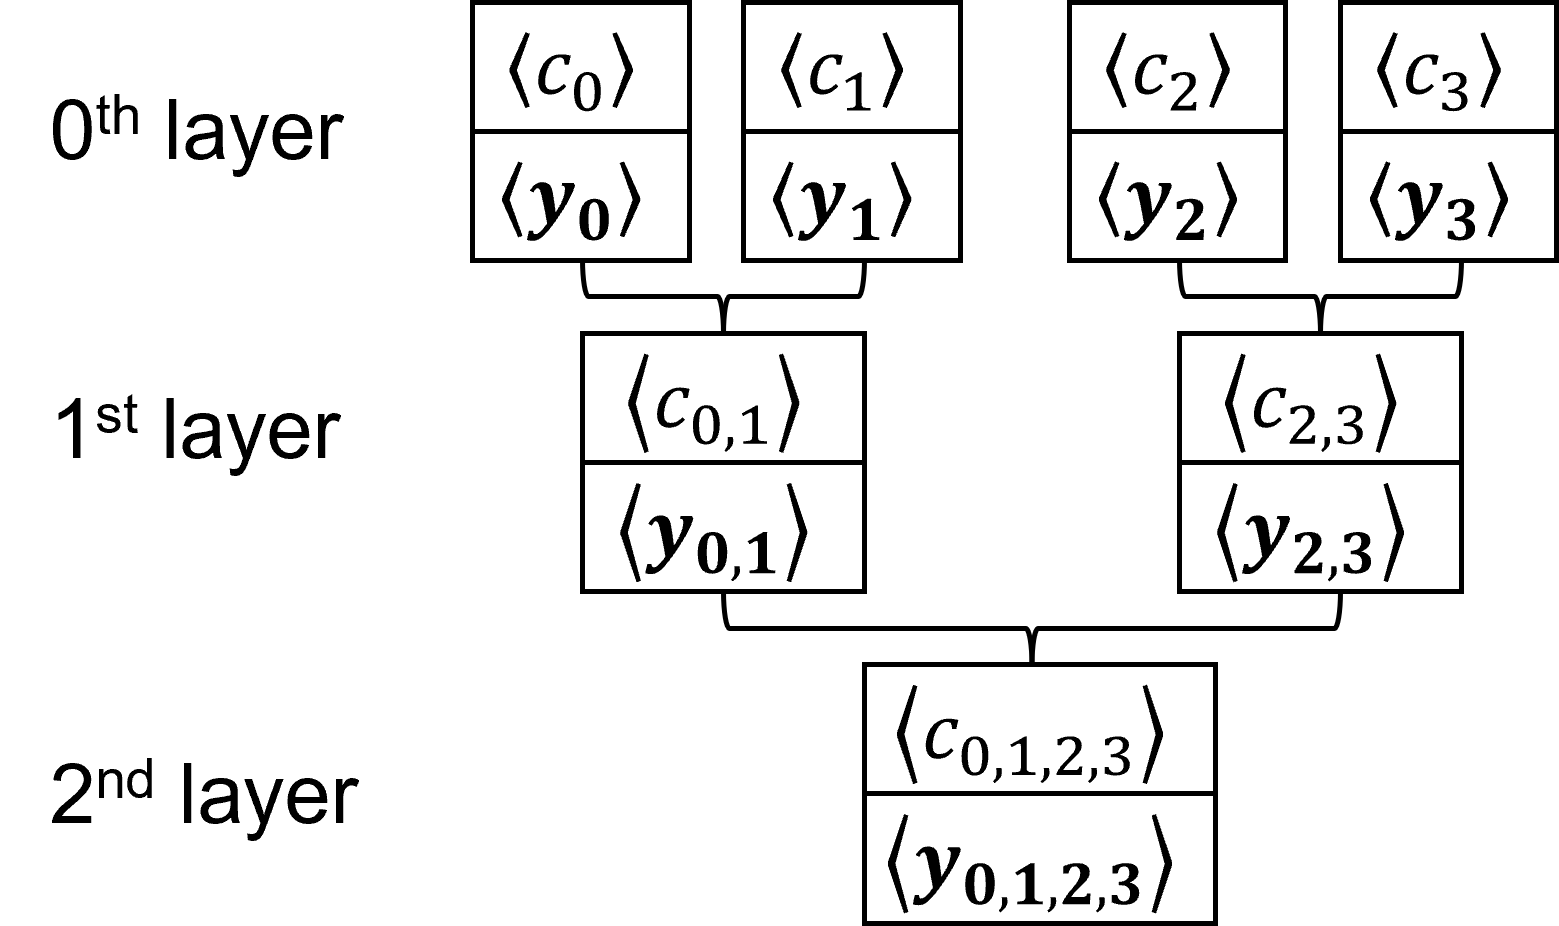
\includegraphics[width=10cm]{ObliviousSelection.png}
    \centering
    \caption{Example inverted binary tree for $\Uppi^{ObliviousSelection}$.}
    \label{img:ObliviousSelection}
\end{figure}
\FloatBarrier


% \subsection{Geometric Distribution}
% \label{prot:GeometricDistribution}
% \autoref{prot:Geometric} is constructed based on $Algo^{Geo}$ (cf.~\autoref{algo:Geometric}). 
% $ \left(u_0,\ldots,u_{iter} \right)\in \left\{0,1\right\}^{iter} $ is a bit string with uniform bits.
% In line $2,3$, we set the bits in $ b_0,\ldots,b_{iter-1}$ to one when the corresponding bits in $u_0,\ldots,u_{iter} $ are the leading zero bits, and other bits in $ b_0,\ldots,b_{iter-1}$ to zero. 
% Recall that the geometric distribution (cf.~\autoref{def:GeometricDistribution}) counts the number of Bernoulli trials up to and including the first success. Therefore, we append bit $1$ and compute the Hamming Weight of string $1, b_0,\ldots,b_{iter-1}$.

% \begin{protocol}[tbh!]
%     \centering
%     \fbox{
%         \pseudocode[space=none, syntaxhighlight=auto, addkeywords={Protocol, Input, Output,FOR,},linenumbering, skipfirstln, head=\textbf{Protocol: $\Uppi^{Geometric}$}]{
%             \textbf{Input: None} \pcskipln \\
%             \textbf{Output: $\left\langle \boldsymbol{y}\right\rangle^{B,UINT}$, where $y\sim Geo\left(p=0.5\right) $} \\
%             \text{$\left(u_0,\ldots,u_{iter-1}\right)  \gets \Uppi^{RandBits}\left(iter\right) $} \\
%             \text{$\left(\left\langle p_{0}\right\rangle^B,\ldots,\left\langle p_{iter-1}\right\rangle^B\right) =\Uppi^{PreOr}\left(\left\langle u_0\right\rangle^B,\ldots, \left\langle u_{iter-1}\right\rangle^B\right) $} \\
%             \text{$\left(\left\langle b_{0}\right\rangle^B,\ldots,\left\langle b_{iter-1}\right\rangle^B\right)  = \left(\operatorname{NOT} \left(\left\langle p_{0} \right\rangle ^B\right),\ldots,\operatorname{NOT} \left(\left\langle p_{iter-1} \right\rangle ^B\right) \right) $} \\
%             % \text{$\left(\left\langle z_0^{ind}\right\rangle^B,\dots,\left\langle z_{iter-1}^{ind}\right\rangle^B\right) =\left(1,\left\langle d_{0}\right\rangle ^B ,\ldots ,\left\langle d_{iter-2}\right\rangle ^B\right) $. }\\
%             \text{$\left\langle \boldsymbol{y}\right\rangle^{B,UINT} =\Uppi^{HW}\left(1,\left\langle b_{0}\right\rangle^B,\ldots,\left\langle b_{iter-2}\right\rangle^B\right) $.}
%         }}
%     \caption{MPC Protocol for geometric distribution $y\sim Geo\left(p=0.5\right)$.}
%     \label{prot:Geometric}
% \end{protocol}
% \FloatBarrier

% % \TODO{explanation}
% \TODO{anaylyse about differential privacy, $iter_2$ leak information of j in second while loop}\\
% \autoref{prot:GeometricExp} converts $Algo^{GeoExp}\left(n,d\right) $ (cf.~\autoref{algo:GeometricExp}) into MPC protocol for $n\neq 0$.
% % We assume two WHILE loop terinates in $iter_1$ and $iter_2$ loops.
% \begin{protocol}[tbh!]
%     \centering
%     \fbox{
%         \pseudocode[space=none, syntaxhighlight=auto, addkeywords={Protocol, Input, Output,FOR,TO},linenumbering, skipfirstln, head=\textbf{Protocol: $\Uppi^{GeometricExp}\left(n,d\right) $ }]{
%             \textbf{Input: $n$, $d$} \pcskipln \\
%             \textbf{Output: $\left\langle \boldsymbol{x}\right\rangle ^{B,UINT} $, where $x \sim Geo\left(p=1-e^{\frac{n}{d}}\right) $} \\
%             % first while loop
%             \text{FOR $j=0$ TO $ iter_1-1$}\\
%             \text{\t\t$\left\langle \boldsymbol{u_j}\right\rangle ^{B,UINT}\gets \Uppi^{RandInt}\left(d\right) $}\\
%             \text{\t\t$\left\langle \boldsymbol{\gamma_{1,j}}\right\rangle ^{B,FX}\gets \frac{\left\langle \boldsymbol{u_j}\right\rangle ^{B,UINT}}{d} $}\\
%             \text{\t\t$\left\langle b_{1,j}\right\rangle ^B=\Uppi^{BernoulliEXP1}\left(\left\langle \boldsymbol{\gamma_{1,j}}\right\rangle ^{B,FX}\right) $ }\\
%             % \text{$\left(\left\langle e_{1,0}\right\rangle ,\ldots,\left\langle e_{1,iter_1-1}\right\rangle \right) =\Uppi^{PreOr}\left(\left\langle b_{1,0}\right\rangle ^B,\ldots,\left\langle b_{1,iter-1}\right\rangle ^B\right) $}\\
%             % \text{For $j \in [1\ldots iter_1)$, parties compute $ \left\langle p^{1}_{j}\right\rangle ^B=\left\langle e^{1}_j\right\rangle^B-\left\langle e^{1}_{j-1}\right\rangle^B$, where $ \left\langle p^{1}_{0}\right\rangle ^B=\left\langle e^{1}_{0}\right\rangle ^B$ }\\
%             % \text{Parties calculate $\left\langle \boldsymbol{u}\right\rangle ^{B,UINT}=\sum_{j=0}^{iter_1-1} \left\langle p^{1}_{j}\right\rangle ^B*\left\langle \boldsymbol{u_j}\right\rangle ^{B,UINT} $}\\
%             % second while loop
%             \text{FOR $k=0$ TO $ iter_2-1$}\\
%             \text{\t\t$\left\langle b_{2,k}\right\rangle ^B=\Uppi^{BernoulliEXP1}\left(1\right) $}\\
%             % \text{$\left(\left\langle e^{2}_{0}\right\rangle ,\ldots,\left\langle e^{2}_{iter_1-1}\right\rangle \right) =\Uppi^{PreOr}\left(\text{NOT}\left(\left\langle b^{2}_{0}\right\rangle ^B\right) ,\ldots,\text{NOT}\left(\left\langle b^{2}_{iter-1}\right\rangle ^B\right) \right) $}\\
%             % \text{For $j \in [1\ldots iter_2)$, parties compute $ \left\langle p^{2}_{j}\right\rangle ^B=\left\langle e^{2}_j\right\rangle^B-\left\langle e^{2}_{j-1}\right\rangle^B$, where $ \left\langle p^{2}_{0}\right\rangle ^B=\left\langle e^{2}_{0}\right\rangle ^B$ }\\
%             % \text{Parties run $\left\langle \boldsymbol{k}\right\rangle ^{B,UINT} =\Uppi^{LeadingZeros}\left(\left\langle p^{2}_{0}\right\rangle ^B,\ldots,\left\langle p^{2}_{iter_2}\right\rangle ^B\right) $}\\
%             % final result
%             % \text{Parties calculate $\left\langle \boldsymbol{x}\right\rangle ^{B,UINT} =\text{FL2UI}\left(\text{Floor}\left(\text{DIV}\left(\text{ADD}\left(\text{MUL}\left(k,d\right), \left\langle \boldsymbol{u}\right\rangle ^{B,UINT}\right),n\right)\right)\right) $}
%             \text{$\left\langle \boldsymbol{u}\right\rangle^{B,UINT}\gets \Uppi^{ObliviousSelection}\left(\left\langle \boldsymbol{u_0}\right\rangle ^{B,UINT},\ldots,\left\langle \boldsymbol{u_{iter_1-1}}\right\rangle ^{B,UINT},\left\langle b_{1,0}\right\rangle ^B,\ldots,\left\langle b_{1,iter_1-1}\right\rangle ^B\right) $}\\
%             \text{$\left\langle \boldsymbol{k}\right\rangle^{B,UINT}\gets \Uppi^{ObliviousSelection}\left(0,\ldots,iter_2-1,\left\langle b_{2,0}\right\rangle ^B,\ldots,\left\langle b_{2,iter_2-1}\right\rangle ^B\right) $}\\
%             \text{$\left\langle \boldsymbol{x}\right\rangle ^{B,UINT}\gets \left\langle \boldsymbol{k}\right\rangle^{B,UINT} \cdot \frac{ d}{n}+\frac{\left\langle \boldsymbol{u}\right\rangle^{B,UINT}}{n}$}
%         }}
%     \caption{MPC Protocol for geometric distribution $x \sim Geo\left(p=1-e^{\frac{n}{d}}\right) $.}
%     \label{prot:GeometricExp}
% \end{protocol}
% \FloatBarrier



% \subsection{Bernoulli Distribution}
% \autoref{prot:Bernoulli} is based on~\autoref{algo:Bernoulli}.
% \begin{protocol}[tbh!]
%     \centering
%     \fbox{
%         \pseudocode[space=none, syntaxhighlight=auto, addkeywords={Protocol, Input, Output},linenumbering, skipfirstln, head=\textbf{Protocol: $\Uppi^{Bernoulli}\left(\left\langle \boldsymbol{p}\right\rangle ^{B,FX} \right) $ }]{
%             \textbf{Input: $\left\langle \boldsymbol{p}\right\rangle ^{B,FX}$} \pcskipln \\
%             \textbf{Output: $\left\langle x\right\rangle ^{B} $, where $x\sim Bern\left(p\right) $} \\
%             \text{$\left\langle \boldsymbol{U}\right\rangle ^{B,UINT} \gets \Uppi^{RandBits}\left(11\right) $}\\
%             \text{$\left\langle \boldsymbol{U}\right\rangle ^{B,FX} \gets \operatorname{UI2FP}\left(\left\langle \boldsymbol{U}\right\rangle ^{B,UINT}\right)  $}\\
%             \text{$\left\langle \boldsymbol{U}\right\rangle ^{B,FX} \gets \operatorname{right-shift}\left(\left\langle \boldsymbol{U}\right\rangle ^{B,FX} ,11\right)  $}\\
%             \text{$\left\langle x\right\rangle^{B} \gets \left(\left\langle p\right\rangle^{B,FX} >\left\langle \boldsymbol{U}\right\rangle ^{B,FX}\right) $}
%         }}
%     \caption{MPC Protocol for Bernoulli distribution $x\sim Bern\left(p\right) $.}
%     \label{prot:Bernoulli}
% \end{protocol}
% \FloatBarrier

% \autoref{prot:BernoulliEXP1} convert $Algo^{BernEXP1}\left(\gamma\right) $~\cite{canonne2020discrete} into MPC protocols. 
% \begin{protocol}[tbh!]
%     \centering
%     \fbox{
%         \pseudocode[space=none, syntaxhighlight=auto, addkeywords={Protocol, Input, Output,FOR},linenumbering, skipfirstln, head=\textbf{Protocol: $\Uppi^{BernoulliEXP1}\left(\left\langle \boldsymbol{\gamma}\right\rangle ^{B,FX}\right) $ }]{
%             \textbf{Input: $\left\langle \boldsymbol{\gamma}\right\rangle ^{B,FX}$} \pcskipln \\
%             \textbf{Output: $\left\langle x\right\rangle ^{B} $, where $x\sim Bern\left(p=e^{-\gamma}\right) $ and $\gamma \in \left[0,1\right] $} \\
%             \text{FOR $j \in [1\ldots iter]$}\\
%             \text{\t\t$\left\langle \boldsymbol{p_j}\right\rangle ^{B,FX}\gets  \frac{\left\langle \boldsymbol{\gamma}\right\rangle ^{B,FX}}{j}  $}\\
%             \text{\t\t$\left\langle b_j\right\rangle ^{B}\gets \Uppi^{Bernoulli}\left(\left\langle \boldsymbol{p_j}\right\rangle ^{B,FX}\right) $}\\
%             \text{\t\t$\left\langle fg_j\right\rangle^{B} \gets \left(\left\langle b_j\right\rangle ^{B}==1\right) $}\\
%             % \text{Parties run $\left(\left\langle e_0\right\rangle^{B} ,\ldots, \left\langle e_{iter}\right\rangle^{B}\right) =\Uppi^{PreOr}\left(\left\langle fg_0\right\rangle^{B},\ldots,\left\langle fg_{iter}\right\rangle^{B}\right) $}\\
%             % \text{For $j \in [1\ldots iter)$, parties compute $ \left\langle p_{j}\right\rangle ^B=\left\langle e_j\right\rangle^B-\left\langle e_{j-1}\right\rangle^B$, where $ \left\langle p_{0}\right\rangle ^B=\left\langle e_{0}\right\rangle ^B$ }\\
%             % \text{Parties compute $\left\langle x \right\rangle^B=\sum_{j = 0}^{iter-1} \left\langle p_{j}\right\rangle ^B*\left\langle b_j\right\rangle ^{B}$}
%             \text{$\left\langle x \right\rangle^B\gets \Uppi^{ObliviousSelection}\left(j_{mod2},\left\langle fg_1\right\rangle^{B},\ldots,\left\langle fg_{iter}\right\rangle^{B}\right) $, where $j_{mod2}=\left(1,0,1,0,\ldots\right) $}
%         }}
%     \caption{MPC Protocol for Bernoulli distribution $x\sim Bern\left(p=e^{-\gamma}\right) $, where $\gamma \in \left[0,1\right] $.}
%     \label{prot:BernoulliEXP1}
% \end{protocol}
% \FloatBarrier


% \autoref{prot:BernoulliEXP} converts $Algo^{BernEXP}\left(\gamma\right) $~\cite{canonne2020discrete} into MPC protocol.
% % We assume that $\gamma<iter$.
% % In line $1,2$, the parties calculate the condition and Bernoulli sampling for the first case.
% % In line $3-13$, the parties calcualte the conditiaon and Bernoulli sampling for the second case. In line $6-8$, the parties extract $b_2==0$ which terminates the for loop under $iter$ iterations. In line $9-12$, the parties calculate the index $j$ where the for loops terminates and compare it with $\left\lfloor \gamma\right\rfloor $ as the condition for case 2.
% % In line $14$, the parties calculate the Bernoulli samples under third case.
% % Finally, the parties calcualte $\left\langle x\right\rangle ^{B} =\left\langle cond_{\gamma \in \left[0,1\right] }\right\rangle ^B*\left\langle b_1\right\rangle ^B+\text{NOT}\left(\left\langle cond_{\gamma \in \left[0,1\right] }\right\rangle ^B\right) *\left(\left\langle cond_{ b2}\right\rangle ^B *\left\langle b_2\right\rangle ^B+\text{NOT}\left(\left\langle cond_{ b2}\right\rangle ^B\right) *\left\langle b_{3}\right\rangle ^B\right) $.

% % Note that the assumption $\gamma<iter$ reveals information about $\gamma$, which implies weaker differential privacy strength.
% % \TODO{anaylyse about differential privacy}\\
% % set the $flag$ to record if the $b_j=1$ is satisfied. In line $5, 6$, the parties calculate the position $p_0,\ldots,p_{iter-1}$ where $p_j=1$ and $j$ is the smallest number such that $flag_j=1$, i.e., the $\text{WHILE}$ loop conditionis not satisfied and algorithms return a result $x=b_j$.\\

% Note that in line $10$, the parties compute $\left\langle x\right\rangle ^B$ with $\left\langle \boldsymbol{b}\right\rangle ^B=\left(\left\langle b_1\right\rangle^B,\left\langle b_{2,0}\right\rangle ^B,\ldots,\left\langle b_{2,iter-1}\right\rangle ^B,\left\langle b_3\right\rangle^B\right) $ and $\left\langle \boldsymbol{fg}     \right\rangle ^{B} =\left(\left\langle cond_{b1}\right\rangle ^B,\left\langle cond_{ b2,0}\right\rangle ^B,\ldots,\left\langle cond_{ b2,iter-1}\right\rangle ^B,1\right)$.


% \begin{protocol}[tbh!]
%     \centering
%     \fbox{
%         \pseudocode[space=none, syntaxhighlight=auto, addkeywords={Protocol, Input, Output,FOR,TO},linenumbering, skipfirstln, head=\textbf{Protocol: $\Uppi^{BernoulliEXP}\left(\left\langle \boldsymbol{\gamma}\right\rangle ^{B,FX}\right) $ }]{
%             \textbf{Input: $\left\langle \boldsymbol{\gamma}\right\rangle ^{B,FX}$} \pcskipln \\
%             \textbf{Output: $\left\langle x\right\rangle ^{B} $, where $x\sim Bern\left(p=e^{-\gamma}\right) $} \\
%             % \gamma \in \left[0,1\right] 
%             % b_1
%             \text{$\left\langle cond_{b1}\right\rangle ^B\gets  \left(\left\langle \boldsymbol{\gamma}\right\rangle ^{B,FX}\leq1\right)   $}\\
%             \text{$\left\langle b_1\right\rangle ^B\gets \Uppi^{BernoulliEXP1}\left(\left\langle \boldsymbol{\gamma}\right\rangle ^{B,FX}\right) $}\\
%             % \gamma >1
%             % b_2
%             \text{$\left\langle \boldsymbol{\left\lfloor \gamma\right\rfloor }\right\rangle ^{B,FX}\gets \operatorname{Floor}\left(\left\langle \boldsymbol{\gamma}\right\rangle ^{B,FX}\right) $}\\
%             \text{FOR $j=0$ TO $ iter-1 $}\\
%             \text{\t\t$\left\langle b_{2,j}\right\rangle ^B \gets \Uppi^{BernoulliEXP1}\left(1\right) $}\\
%             \text{\t\t$\left\langle cond_{b_{2,j}==0}\right\rangle ^B \gets \left(\left\langle b_{2,j}\right\rangle ^B ==0\right) $}\\
%             % \text{$\left(\left\langle e_{0}\right\rangle ,\ldots,\left\langle e_{iter-1}\right\rangle \right) =\Uppi^{PreOr}\left(\left\langle b_{0,2}\right\rangle ^B,\ldots,\left\langle b_{iter-1,2}\right\rangle ^B\right) $}\\
%             % \text{For $j \in [1\ldots iter)$, parties compute $ \left\langle p_{j}\right\rangle ^B=\left\langle e_j\right\rangle^B-\left\langle e_{j-1}\right\rangle^B$, where $ \left\langle p_{0}\right\rangle ^B=\left\langle e_{0}\right\rangle ^B$ }\\
%             % \text{Parties calculate $\left\langle b_2\right\rangle ^B=\sum_{j=0}^{iter-1} \left\langle p_{j}\right\rangle ^B*\left\langle b_{j,2}\right\rangle ^B $}\\
%             % \text{Parties calculate $\left\langle \boldsymbol{j_{b_{j,2}==0}}\right\rangle ^{B,UINT}=\Uppi^{LeadingZeros}\left(\left\langle p_{0}\right\rangle ^B,\ldots,\left\langle p_{iter-1}\right\rangle ^B\right) $}\\
%             % \text{Parties calcualte $\left\langle \boldsymbol{\left\lfloor \gamma\right\rfloor }\right\rangle ^{B,UINT}=\text{FL2UI}\left(\left\langle \boldsymbol{\left\lfloor \gamma\right\rfloor }\right\rangle ^{B,FL}\right) $}\\
%             \text{\t\t$\left\langle cond_{ b2,j}\right\rangle ^B \gets \left(j< \left\langle \boldsymbol{\left\lfloor \gamma\right\rfloor }\right\rangle ^{B,FX}\right)  \land \left\langle cond_{b_{2,j}==0}\right\rangle ^B  $}\\
%             % b_3
%             \text{$\left\langle \boldsymbol{\gamma-\left\lfloor \gamma\right\rfloor }\right\rangle ^{B,FX}\gets \left\langle \boldsymbol{\gamma}\right\rangle ^{B,FX} -\left\langle \boldsymbol{\left\lfloor \gamma\right\rfloor }\right\rangle ^{B,FX}$}\\
%             \text{$\left\langle b_{3}\right\rangle ^B =\Uppi^{BernoulliEXP1}\left(\left\langle \boldsymbol{\gamma-\left\lfloor \gamma\right\rfloor }\right\rangle ^{B,FL}\right) $}\\
%             % final result
%             \text{$ \left\langle x\right\rangle ^{B} \gets \Uppi^{ObliviousSelection}\left(\left\langle \boldsymbol{b}\right\rangle ^B, \left\langle \boldsymbol{fg}     \right\rangle ^{B}   \right) $}
%         }}
%     \caption{MPC Protocol for Bernoulli distribution $x\sim Bern\left(p=e^{-\gamma}\right) $.}
%     \label{prot:BernoulliEXP}
% \end{protocol}
% \FloatBarrier

% \subsection{Random Integer}
% \autoref{prot:RandInt} convert $Algo^{RandInt}\left(m\right)$ into MPC protocol.\\
% \TODO{Problem with unsigned integer because $\kappa$ is requires be greater than 64.}\\
% \begin{protocol}[tbh!]
%     \centering
%     \fbox{
%     \pseudocode[space=none, syntaxhighlight=auto, addkeywords={Protocol, Input, Output},linenumbering, skipfirstln, head=\textbf{Protocol: $\Uppi^{RandInt}\left(m\right) $ }]{
%     \textbf{Input: $m$} \pcskipln \\
%     \textbf{Output: $\left\langle \boldsymbol{x}\right\rangle ^{B,UINT} $, where $x \in [0,m) $} \\
%     \text{$\left\langle \boldsymbol{r}\right\rangle ^{B,UINT} \gets \Uppi^{RandBits}\left(l+kappa\right)$ }\\
%     \text{$\left\langle \boldsymbol{x}\right\rangle^{B,UINT} \gets \text{MOD}\left(\left\langle \boldsymbol{r}\right\rangle ^{B,UINT},m\right) $}
%     }}
%     \caption{MPC Protocol for random integer $x \sample [0,m) $.}
%     \label{prot:RandInt}
% \end{protocol}
% \FloatBarrier








% % Protocol $\Uppi^{LeadingZeros}\left(\left\langle \boldsymbol{s} \right\rangle^B,l\right) $ counts the number of leading zeros in a $l$-bit string $\boldsymbol{s}$. We apply $\Uppi^{PreOr} $ to find the position $e$ of the first appearance of one in string $\boldsymbol{s}$. Finally, by inverting $e$, we get $e_j=1$ if $s_j$ belongs to the leading zeros. In line $3$, we convert boolean share to arithmetic share to count the total number of leading zeros (number of $d_j\neq 0$).\\
% % \begin{protocol}[tbh!]
% %     \centering
% %     \fbox{
% %     \pseudocode[space=none, syntaxhighlight=auto, addkeywords={Protocol, Input, Output},linenumbering, skipfirstln, head=\textbf{Protocol: $\Uppi^{LeadingZeros}\left(\left\langle \boldsymbol{s}\right\rangle^B,l\right) $}]{
% %     \textbf{Input: $l$-bit string $\left\langle \boldsymbol{s}\right\rangle^B$ } \pcskipln \\
% %     \textbf{Output: $\left\langle z\right\rangle^A$} \\
% %     \text{Parties run $\Uppi^{PreOr}\left(\left\langle \boldsymbol{s} \right\rangle^B\right) $ and obtain $\left\langle e_{j}\right\rangle^B$. } \\
% %     \text{For $j \in [0\ldots l)$, parties compute $\left\langle d_j\right\rangle^B=\text{NOT}\left(\left\langle e_{j}\right\rangle^B\right) in parallel$. }\\
% %     \text{Parties compute $\left\langle \boldsymbol{z}\right\rangle^{B,UINT}=\sum_{j = 0}^{l-1}\text{B2A}\left(\left\langle d_{j}\right\rangle^B \right) $. }
% %     }}
% %     \caption{MPC Protocol for counting leading zeros.}
% %     \label{prot:LeadingZeros}
% % \end{protocol}
% % \FloatBarrier

% % Protocol $\Uppi^{BitsContainOne}\left(\left\langle \boldsymbol{s} \right\rangle^B,l\right) $ outputs $o=1$ if the given $l$-bit string $\boldsymbol{s}$ contains one, and $o=0$ otherwise.\\
% % \begin{protocol}[tbh!]
% %     \centering
% %     \fbox{
% %         \pseudocode[space=none, syntaxhighlight=auto, addkeywords={Protocol, Input, Output},linenumbering, skipfirstln, head=\textbf{Protocol: $\Uppi^{BitsContainOne}$}]{
% %             \textbf{Input: $l$-bit string $\left\langle \boldsymbol{s}\right\rangle^B$ } \pcskipln \\
% %             \textbf{Output: $\left\langle o\right\rangle^B$} \\
% %             \text{Parties compute $\left\langle o\right\rangle ^B=\lor _{j=0}^{l}\left\langle s_{j}\right\rangle^B$ }
% %         }}
% %     \caption{MPC Protocol for checking if $l$-bit string $s$ contains one.}
% %     \label{prot:BitsContainOne}
% % \end{protocol}
% % \FloatBarrier

% \subsection{Binary2Unary}

% \TODO{Binary2Unary needs to be improved.}
% $\Uppi^{Binary2Unary}\left(\left\langle a\right\rangle^A ,l\right) $~\cite{aliasgari2012secure} converts integer $a$ from binary to unary bitwise representation and outputs a $l$-bit string $\boldsymbol{p}=\left( p_{0} ,\ldots , p_{l-1} \right) $, where the $a$ least significant bits $\left( p_{0} ,\ldots , p_{a-1} \right)$ are set to $1$ and others to $0$. In line $1,2$, we calculate the $2^a$ and convert it to boolean shares. Then in line $3$ we generate $l+k$ random bits and hide $2_a$ by adding it with the $l+k-1$-bit integer and reconstruct the addition result $c$. In line $5$, the plaintext value $c$ is decomposed into binary bits. In line $6$, we compute $XOR$ of $c_j$ and correspond bit $u_j$. Then in line $7$, by $PreOr$ we get $\left(g_{l-1},\ldots,g_j\right) =\left(\overline{1}_{\left(l-j+1\right) }\right) $ and $\left(g_{j-1},\ldots,g_{0}\right) =\left(\overline{0}_{\left(j\right) }\right) $, where $j-1=a$. Finally, we calculate $\left(p_{l-1},\ldots,p_{0}\right)=\text{NOT}\left(g_{l-1},\ldots,g_{0}\right) $ and the number of non-zero bits in $\left(p_{l-1},\ldots,p_{0}\right)$ equals to $a$. The share conversion in line $4$ can be omitted if arithmetic of boolean shares is available.\\
% \begin{protocol}[tbh!]
%     \centering
%     \fbox{
%     \pseudocode[space=none, syntaxhighlight=auto, addkeywords={Protocol, Input, Output},linenumbering, skipfirstln, head=\textbf{Protocol: $\Uppi^{Binary2UnaryOld}\left(\left\langle a\right\rangle^A ,l\right) $}]{
%     \textbf{Input: $\left\langle \boldsymbol{a}\right\rangle^B $, $l$} \pcskipln \\
%     \textbf{Output: $\left\langle p_{0}\right\rangle ^B,\ldots ,\left\langle p_{l-1}\right\rangle^B $} \\
%     \text{Parties compute $\left\langle \boldsymbol{2^{a}}\right\rangle ^B=\text{Pow2}\left(\left\langle a\right\rangle ^A,l\right) $} \\
%     \text{Parties compute $ \left\langle 2^{a}\right\rangle ^A=\text{B2A}\left(\left\langle \boldsymbol{2^{a}} \right\rangle ^B\right) $} \\
%     \text{Parties run $\Uppi^{RandBits}\left(l+k\right) $ and obtain $\left\langle u_0\right\rangle ^B,\ldots,\left\langle u_{l+k-1}\right\rangle ^B$.} \\
%     % \text{Parties reconstruct $c \gets \text{Rec}\left(\left\langle 2^{a}\right\rangle^A+2^{l}*\text{B2A}\left(\left\langle u_{l+k-1}\right\rangle ^B,\ldots, \left\langle u_l\right\rangle ^B\right) + \text{B2A}\left(\left\langle u_{l-1}\right\rangle^B,\ldots,\left\langle u_0\right\rangle^B \right) \right) $} \\
%     \text{Parties reconstruct $c \gets \text{Rec}\left(\left\langle 2^{a}\right\rangle^A + \text{B2A}\left(\left\langle u_{l+k-1}\right\rangle^B,\ldots,\left\langle u_0\right\rangle^B \right) \right) $} \\
%     \text{Each party locally run $\Uppi^{Bits}\left(c,l\right) $ and obtain $\left(c_{0},\ldots ,c_{l-1}\right) $} \\
%     \text{For $j\in\left[0 \ldots l\right) $, each party locally compute $\left\langle t_j\right\rangle^B =\text{XOR}\left(c_j,\left\langle u_j\right\rangle ^B\right) $} \\
%     \text{For $j\in\left[0 \ldots l\right) $, parties compute $\Uppi^{PreOr}\left(\left\langle t_0\right\rangle^B,\ldots, \left\langle t_l\right\rangle^B\right) $ and obtain $\left\langle g_0\right\rangle^B,\ldots, \left\langle g_l\right\rangle^B$}\\
%     \text{For $j\in\left[0 \ldots l\right) $, parties compute $\left\langle p_j\right\rangle^B =\text{NOT}\left(\left\langle g_j\right\rangle ^B\right) $}
%     }}
%     \caption{MPC Protocol for binary to unary conversion.}
%     \label{prot:Binary2Unary}
% \end{protocol}
% \FloatBarrier

% \begin{protocol}[tbh!]
%     \centering
%     \fbox{
%         \pseudocode[space=none, syntaxhighlight=auto, addkeywords={Protocol, Input, Output},linenumbering, skipfirstln, head=\textbf{Protocol: $\Uppi^{Binary2UnaryNEW}\left(\left\langle \boldsymbol{a}\right\rangle^{B,UINT} ,l\right) $}]{
%             \textbf{Input: $\left\langle \boldsymbol{a}\right\rangle^{B,UINT} $, $l$} \pcskipln \\
%             \textbf{Output: $\left\langle p_{0}\right\rangle ^B,\ldots ,\left\langle p_{l-1}\right\rangle^B $} \\
%             \text{Parties compute $\left\langle \boldsymbol{t}\right\rangle ^{B,UINT}=\text{POW2}\left(\left\langle \boldsymbol{a}\right\rangle ^{B,UINT}\right) $.} \\
%             \text{Parties compute $\left(\left\langle e_0\right\rangle^B,\ldots,\left\langle e_{64-1}\right\rangle^B\right) =\Uppi^{PreOr}\left(\left\langle t_0\right\rangle^B,\ldots,\left\langle t_{64-1}\right\rangle^B\right) $.} \\
%             \text{Each party locally set $\left\langle p_0\right\rangle^B=\text{NOT}\left(\left\langle e_0\right\rangle^B\right) ,\ldots,\left\langle p_{l-1}\right\rangle^B=\text{NOT}\left(\left\langle e_{l-1}\right\rangle^B\right) $.}
%         }}
%     \caption{MPC Protocol for binary to unary conversion.}
%     \label{prot:Binary2Unary}
% \end{protocol}
% \FloatBarrier




% % \begin{protocol}[tbh!]
% %     \centering
% %     \fbox{
% %         \pseudocode[space=none, syntaxhighlight=auto, addkeywords={Protocol, Input, Output},linenumbering, skipfirstln, head=\textbf{Protocol: $\Uppi^{Split}\left(\left\langle \boldsymbol{L}\right\rangle^{B,UINT} ,\left\langle \boldsymbol{R}\right\rangle ^{B,UINT} ,\lambda\right) $}]{
% %             \textbf{Input: $\left\langle \boldsymbol{L}\right\rangle^{B,UINT}$, $\left\langle \boldsymbol{R}\right\rangle ^{B,UINT}$, $\lambda$} \pcskipln \\
% %             \textbf{Output: $\left\langle \boldsymbol{M}\right\rangle^{B,UINT}$, where $M=L-\text{int}\left(\frac{\ln\left(0.5\right)+\ln\left(1+e^{-\lambda\left(R-L\right) }\right) }{\lambda}\right)$} \\
% %             \text{Parties compute $\left\langle \boldsymbol{t}\right\rangle ^{B,FL}=\frac{\text{LN}\left(0.5\right)+\text{LN}\left(1+\text{EXP}\left(-\lambda \cdot \left(\left\langle \boldsymbol{R}\right\rangle ^{B,UINT}-\left\langle \boldsymbol{L}\right\rangle^{B,UINT}\right)\right) \right) }{\lambda}$.}\\
% %             \text{Parties compute $\left\langle \boldsymbol{M}\right\rangle^{B,UINT}=\left\langle \boldsymbol{L}\right\rangle^{B,UINT}-\text{FL2UI}\left(\left\langle \boldsymbol{t}\right\rangle ^{B,FL}\right) $.}
% %         }}
% %     \caption{MPC Protocol for $\text{Split}\left(L,R,\lambda\right)=L-\text{int}\left(\frac{\ln\left(0.5\right)+\ln\left(1+e^{-\lambda\left(R-L\right) }\right) }{\lambda}\right) $.}
% %     \label{prot:Split}
% % \end{protocol}
% % \FloatBarrier

% % \begin{protocol}[tbh!]
% %     \centering
% %     \fbox{
% %         \pseudocode[space=none, syntaxhighlight=auto, addkeywords={Protocol, Input, Output},linenumbering, skipfirstln, head=\textbf{Protocol: $\Uppi^{Proportion}\left(\left\langle \boldsymbol{L_{j-1}}\right\rangle^{B,UINT} ,\left\langle \boldsymbol{R_{j-1}}\right\rangle ^{B,UINT} ,\left\langle \boldsymbol{M_j}\right\rangle ^{B,UINT} ,\lambda\right)$}]{
% %             \textbf{Input: $\left\langle \boldsymbol{L}\right\rangle^{B,UINT}$, $\left\langle \boldsymbol{R}\right\rangle ^{B,UINT}$, $\left\langle \boldsymbol{M}\right\rangle^{B,UINT}$, $\lambda$} \pcskipln \\
% %             \textbf{Output: $\left\langle \boldsymbol{Q}\right\rangle ^{B,FL}$, where $Q=\frac{e^{-\lambda\left(M-L\right) }-1}{e^{-\lambda\left(R-L\right) }-1} $} \\
% %             \text{Parties compute $\left\langle \boldsymbol{Q}\right\rangle ^{B,FL}=\frac{e^{-\lambda \cdot \left(\left\langle \boldsymbol{M}\right\rangle ^{B,FL}-\left\langle \boldsymbol {L}\right\rangle ^{B,FL}\right) }-1}{e^{-\lambda \cdot \left(\left\langle \boldsymbol{R}\right\rangle ^{B,FL}- \left\langle \boldsymbol{L}\right\rangle ^{B,FL}\right) }-1} $.}
% %         }}
% %     \caption{MPC Protocol for $\text{Proportion}\left(L,R,M,\lambda\right)=\frac{e^{-\lambda\left(M-L\right) }-1}{e^{-\lambda\left(R-L\right) }-1} $.}
% %     \label{prot:Proportion}
% % \end{protocol}
% % \FloatBarrier





% % \begin{algorithm}[tbh!]
% %     \centering
% %     \fbox{
% %     \pseudocode[space=none, syntaxhighlight=auto, addkeywords={Protocol, Input, Output},linenumbering, head=\textbf{Function $\text{AGT}\left(\left\langle x_0\right\rangle^A, \left\langle x_1\right\rangle^A,\ell_s \right)  $}]{
% %     \text{$\left\langle \delta \right\rangle^A=\left\langle x_1\right\rangle^A-\left\langle x_0\right\rangle^A $}\\
% %     \text{$\ell_{prev}=1$}\\
% %     \text{if $\ell>\ell_s$ then}\\
% %     \text{\t\t if $\ell==\ell_s+2$ then}\\
% %     \text{\t\t \t\t $\ell_s=\ell_s+1$}\\
% %     \text{\t\t $sel \gets\left\langle \delta \right\rangle^A_0\left[1:\ell_s\right] $ }\\
% %     \text{\t\t     $M  \gets\left(j+\langle\delta\rangle_{1}^{A}\left[1: \ell_{s}\right]>2^{\ell_{s}}\right)_{j=1}^{2^{\ell_s}} $ }\\
% %     \text{\t\t $r  \sample \left\{0,1\right\} $}\\
% %     \text{\t\t $c\gets \binom{N}{1} \text{-OT}\left(sel,\left\{m\oplus r\right\}_{m\in M} \right) $}\\
% %     \text{\t\t $\ell_{prev}\gets \ell_s+1$}\\
% %     \text{while $\ell_{prev} < \ell-1$}\\
% %     \text{\t\t $\ell_{s}^{\prime} \gets \min \left(\ell_{s}-1, \ell-\ell_{prev }-1\right)$}\\
% %     \text{\t\t $\ell_ {next }\gets \ell_ {prev }+\ell_{s}^{\prime}$}\\
% %     \text{\t\t if $\ell_{next}+2==\ell$ then}\\
% %     \text{\t\t \t\t $\ell_{next}=\ell_{next}+1$}\\
% %     \text{\t\t $ sel \gets \left\langle \delta\right\rangle_{0} ^{A}  \left[\ell_{prev}: \ell_{next }\right] .$}\\
% %     \text{\t\t $sel\gets sel+c\cdot 2^{\ell_s^{\prime}+1}$}\\
% %     \text{\t\t $\left\langle\delta^{\prime}\right\rangle_{1}^{A} \gets\langle\delta\rangle_{1}^{A}\left[\ell_{prev }: \ell_{next }\right]$}\\
% %     \text{\t\t $M_{0} \gets\left\{j+\left\langle\delta^{\prime}\right\rangle_{1}^{A}>2^{\ell_{s}^{\prime}+1}\right\}_{j=1}^{2^{\ell_s^{\prime}+1}}$}\\
% %     \text{\t\t $M_{1} \gets\left\{j+\left\langle\delta^{\prime}\right\rangle_{1}^{A}+1>2^{\ell_{s}^{\prime}+1}\right\}_{j=1}^{2^{\ell_s^{\prime}+1}}$}\\
% %     \text{\t\t $M \gets M_{r} \cup M_{1-r}$}\\
% %     \text{\t\t $r \sample \left\{0,1\right\} $}\\
% %     \text{\t\t $c\gets \binom{N}{1} \text{-OT}\left(sel,\left\{m\oplus r\right\}_{m\in M} \right) $}\\
% %     \text{\t\t $\ell_{prev } \gets \ell_{next }+1$}\\
% %     \text{$\left\langle b\right\rangle^B=\left(\left\langle b\right\rangle_0^B, \left\langle b\right\rangle_1^B\right):=\left(c\oplus \left\langle \delta \right\rangle^A_0\left[\ell\right]  ,r\oplus\left\langle \delta \right\rangle^A_1\left[\ell\right] \right)  $}\\
% %     \text{return $\left\langle b\right\rangle^B $}
% %     }}
% % \end{algorithm}
% % \FloatBarrier


% % \section{MPC Techniques}
% % \label{sec:MPCTechniques}
% % We applied certain techniques to convert algorithms into computations of MPC.

% % \subsection{Branching}
% % We convert \textbf{IF} branching in algorithm $Algo^{Branching}$~\autoref{algo:Branching} into MPC computations as

% % \[\text{output}=\left\langle a\right\rangle^B \land \left\langle b\right\rangle ^B \oplus  \text{NOT}\left(\left\langle a\right\rangle ^B\right) \land \left\langle c\right\rangle^B . \]

% % \begin{algorithm}[tbh!]
% %     \centering
% %     \fbox{
% %         \pseudocode[space=none, syntaxhighlight=auto, addkeywords={Protocol, Input, Output, IF, ELSE, RETURN},linenumbering, skipfirstln, head=\textbf{Protocol: $Algo^{Branching}$}]{
% %             % \textbf{Input: $\left\langle e\right\rangle^A $} \pcskipln \\
% %             % \textbf{Output: $\left( \left\langle y_{1}\right\rangle ^B, \ldots, \left\langle y_{11} \right\rangle ^B \right)$, $\left\langle y\right\rangle ^A$} \\
% %             \text{$\ldots$} \\
% %             \text{IF $\left\langle a\right\rangle^B $ }\\
% %             \text{\t\t RETURN $\left\langle b\right\rangle^B $}\\
% %             \text{ELSE}\\
% %             \text{\t\t RETURN $\left\langle c\right\rangle ^B$}\pcskipln\\
% %             \text{$\ldots$}
% %         }}
% %     \caption{Algorithm example with \textbf{IF} branching.}
% %     \label{algo:Branching}
% % \end{algorithm}
% % \FloatBarrier


% % \subsection{Loop}
% % Suppose $Algo^{Lottery}$~\autoref{algo:Lottery} is a lottery algorithm (charging $b$ amount of money for each draw) that you can draw unlimited times , and the reward $r$ decreases as the number of draws increases. $Algo^{Toss}$ output either $1$ (win) or $0$ (lose) with the same probability $p=0.5$.

% % \begin{algorithm}[tbh!]
% %     \centering
% %     \fbox{
% %         \pseudocode[space=none, syntaxhighlight=auto, addkeywords={Protocol, Input, Output, IF, ELSE, RETURN, WHILE, TRUE},linenumbering, skipfirstln, head=\textbf{Algorithm: $Algo^{Lottery}$}]{
% %             \text{$\ldots$} \\
% %             \text{$trials\gets 0$}\\
% %             \text{WHILE TRUE }\\
% %             \text{\t\t $  a \gets Algo^{Toss}\left(  b \right) $}\\
% %             \text{\t\t IF $a$}\\
% %             \text{\t\t \t\t RETURN $r-trials$}\\
% %             \text{\t\t $trials\gets trials+1$} \pcskipln \\
% %             \text{$\ldots$}
% %         }}
% %     \caption{Algorithm example with \textbf{WHILE} loop.}
% %     \label{algo:Lottery}
% % \end{algorithm}
% % \FloatBarrier

% % To transform $Algo^{Lottery}$ into MPC computations, the parties first assume that they will get the reward (i.e., \textbf{WHILE} loop terminates when $\left\langle a_j\right\rangle^{B}==1 $ for the first time) after $iter$ trials with very high probability. Then, the parties run $\Uppi^{Toss}$ for $iter$ times to compute $\left\langle a_j\right\rangle^{B} $ for $j \in [0\ldots iter)$. Since they don't know when $\left\langle a_j\right\rangle^{B}==1 $ happens for the first time, they run $\Uppi^{PreOr}$ in line $4$ to calculate $e_j=\lor_{k=0}^{j}a_{k}$ such that $e_0=0,\ldots,e_{s-1}=0$ and $e_s=1,\ldots,e_{iter-1}=1$, where $s$ is the smallest index in the interval $ [0\ldots iter)$ making $\left\langle a_j\right\rangle^{B}==1 $. In line $6$, they calculate and get $p_s=1$, $p_t=0$ for $t \in [0\ldots iter)\setminus s$. Finally, the parties $\text{AND}$ the reward of each iteration with $p_j$ for $j \in [0\ldots iter)$ and $\text{XOR}$ these values to extract the correct reward $x$.

% %             \begin{protocol}[tbh!]
% %                 \centering
% %                 \fbox{
% %                     \pseudocode[space=none, syntaxhighlight=auto, addkeywords={Protocol, Input, Output, IF, ELSE, RETURN, WHILE, TRUE, FOR, TO},linenumbering, skipfirstln, head=\textbf{Protocol: $\Uppi^{Lottery}$}]{
% %                         \text{$\ldots$} \\
% %                         \text{Each party locally set $trial=0$.}\\
% %                         \text{FOR $j=0$ TO $iter-1$ }\\
% %                         \text{\t\t Parties run $\left\langle a_j\right\rangle^{B}= \Uppi^{Toss}\left(\left\langle \boldsymbol{b}\right\rangle^{B,UINT }\right) $.}\\
% %                         \text{Parties compute $\left(\left\langle e_0\right\rangle^B,\ldots,\left\langle e_{iter-1}\right\rangle^B\right) =\Uppi^{PreOr}\left(\left\langle a_0\right\rangle^B,\ldots,\left\langle a_{iter-1}\right\rangle^B\right) $.}\\
% %                         \text{FOR $j=0$ TO $iter-1$ }\\
% %                         \text{\t\t Each party locally compute $ \left\langle p_{j}\right\rangle ^B=\left\langle e_j\right\rangle^B \oplus \left\langle e_{j-1}\right\rangle^B$, where $ \left\langle p_{0}\right\rangle ^B=\left\langle e_{0}\right\rangle ^B$.} \\
% %                         \text{Parties compute $\left\langle x\right\rangle^{B,UINT}=\oplus_{j=0}^{iter-1}\left\langle p_{j}\right\rangle ^B \land \left(\left\langle \boldsymbol{r}\right\rangle^{B,UINT}-j\right) $.}\pcskipln \\
% %                         \text{$\ldots$}
% %                     }}
% %                 \caption{MPC protocol for algorithm with \textbf{WHILE} loop.}
% %                 \label{prot:Lottery}
% %             \end{protocol}
% %             \FloatBarrier





% \section{Additional Proof}
% \label{sec:additionalProof}

% % \subsection{Proofs of Equations in \autoref{algo:GeometricExpBinarySearch}}

% \subsubsection{Function $\operatorname{Split}\left(L,R,\lambda\right)$}
% \label{subsubsec:Split}

% Function $\text{Split}\left(L,R,\lambda\right)=L-\text{int}\left(\frac{\ln\left(0.5\right)+\ln\left(1+e^{-\lambda\left(R-L\right) }\right) }{\lambda}\right)$ calculates the middle point $M$ of interval $\left(L\ldots R\right] $ such that for $Geo\left(p=1-e^{-\lambda}\right) $'s PMF
% \[\text{Pr}\left(L< x \leq M \, | \, L < x\leq R\right)\approx \frac{1}{2}.\]

% First, we calculate $ \text{Pr}\left(L< x \leq M \right)$ and $ \text{Pr}\left(L< x \leq R \right)$ as follows:
% \begin{equation}
%     \begin{split}
%         \text{Pr}\left(L< x \leq M \right)&=\text{Pr}\left(x \leq M \right)-\text{Pr}\left( x \leq L \right)\\
%         & =\left(1-\left(1-p\right)^M\right) -\left(1-\left(1-p\right)^L\right)\\
%         & =\left(1-e^{-\lambda M}\right) -\left(1-e^{-\lambda L}\right)\\
%         & =e^{-\lambda L}-e^{-\lambda M}\\
%         &=\frac{1}{e^{\lambda L}}-\frac{1}{e^{\lambda M}}\\
%         & =\frac{e^{\lambda M}-e^{\lambda L}}{e^{\lambda L+\lambda M}},\\
%     \end{split}
% \end{equation}

% \begin{equation}
%     \begin{split}
%         \text{Pr}\left(L< x \leq R \right)&=\text{Pr}\left(x \leq R \right)-\text{Pr}\left( x \leq L \right)\\
%         & =\left(1-\left(1-p\right)^R\right) -\left(1-\left(1-p\right)^L\right)\\
%         & =\left(1-e^{-\lambda R}\right) -\left(1-e^{-\lambda L}\right)\\
%         & =e^{-\lambda L}-e^{-\lambda R}\\
%         &=\frac{1}{e^{\lambda L}}-\frac{1}{e^{\lambda R}}\\
%         &=\frac{e^{\lambda R}-e^{\lambda L}}{e^{\lambda L+\lambda R}}.
%     \end{split}
% \end{equation}

% Then, we calculate $\text{Pr}\left(L< x \leq M \, | \, L < x\leq R\right)  $ as follows:
% \begin{equation}
%     \begin{split}
%         \text{Pr}\left(L< x \leq M \, | \, L < x\leq R\right) &=\frac{\text{Pr}\left(L< x \leq M \right)}{\text{Pr}\left(L< x \leq R \right)}\\
%         &=\frac{e^{\lambda M}-e^{\lambda L}}{e^{\lambda L+\lambda M}}\cdot \frac{e^{\lambda L+\lambda R}}{e^{\lambda R}-e^{\lambda L}}\\
%         &=\frac{e^{\lambda M}-e^{\lambda L}}{e^{\lambda R}-e^{\lambda L}}\cdot e^{\lambda \left(R-M\right) }\\
%         &=\frac{e^{\lambda R }-e^{\left(L+R-M\right) }}{e^{\lambda R}-e^{\lambda L}}.
%     \end{split}
% \end{equation}

% Finally, we calculate the value middle point $M$ such that $\text{Pr}\left(L< x \leq M \, | \, L < x\leq R\right)  \approx  \frac{1}{2}$ as follows:
% \begin{equation}
%     \begin{split}
%         \text{Pr}\left(L< x \leq M \, | \, L < x\leq R\right) & \approx  \frac{1}{2} \\
%         \frac{e^{\lambda R }-e^{\lambda\left(L+R-M\right) }}{e^{\lambda R}-e^{\lambda L}} & \approx \frac{1}{2} \\
%         e^{\lambda R }-e^{\lambda\left(L+R-M\right) }& \approx  \frac{1}{2} \left(e^{\lambda R}-e^{\lambda L}\right) \\
%         \frac{1}{2} \left(e^{\lambda R} +  e^{\lambda L}\right)    & \approx    e^{\lambda\left(L+R-M\right) }    \\
%         \ln \left( \frac{1}{2} \left(e^{\lambda R} +  e^{\lambda L}\right)\right) & \approx  \ln \left( e^{\lambda\left(L+R-M\right) }\right)       \\
%         \ln \left( \frac{1}{2}\right) +\ln\left(e^{\lambda R} +  e^{\lambda L}\right)  & \approx \lambda \left(L+R-M\right)        \\
%         \ln \left( \frac{1}{2}\right) +\ln\left(e^{\lambda R} +  e^{\lambda L}\right)  & \approx \ln\left(e^{\lambda R}\right) +\lambda \left(L-M\right)        \\
%         \ln \left( \frac{1}{2}\right) +\ln\left(e^{\lambda R} +  e^{\lambda L}\right) -\ln\left(e^{\lambda R}\right) & \approx  \lambda\left(L -M\right)       \\
%         \ln \left( \frac{1}{2}\right) +\ln\left(\frac{e^{\lambda R} +  e^{\lambda L}}{e^{\lambda R}}\right)  & \approx \lambda \left(L -M \right)      \\
%         \ln \left( \frac{1}{2}\right) +\ln\left(1+e^{-\lambda\left(R-L\right) }\right)  & \approx  \lambda\left(L -M\right)       \\
%         \frac{\ln \left( \frac{1}{2}\right) +\ln\left(1+e^{-\lambda\left(R-L\right) }\right)} {{\lambda }} & \approx  L -M      \\
%         L- \frac{\ln \left( \frac{1}{2}\right) +\ln\left(1+e^{-\lambda\left(R-L\right) }\right)} {{\lambda }} & \approx  M      \\
%     \end{split}
% \end{equation}



%     % calculates the proportion $Q$ of $\text{Pr}\left(L< x \leq M \right)$ and $\text{Pr}\left(L< x \leq R \right)$ regarding $Geo\left(p=1-e^{-\lambda}\right) $'s PMF, that is defined as follows:

%     % \begin{equation}
%     %     \begin{split}
%     %         Q & =\text{Pr}\left(L< x \leq M \, | \, L < x\leq R\right)\\
%     %         & =\frac{\text{Pr}\left(L< x \leq M \right)}{\text{Pr}\left(L< x \leq R \right)}\\
%     %         &=\ldots\\
%     %         &= \frac{e^{-\lambda\left(M-L\right) }-1}{e^{-\lambda\left(R-L\right) }-1}
%     %     \end{split}
%     % \end{equation}